%!TEX root = ./icml2016.tex
\section{Experiments}
\subsection{Synthetic data}
\begin{figure}[t]
	\centering
	
	\subfigure[E=5, K=5, D=5\label{fig:syn1}]{
	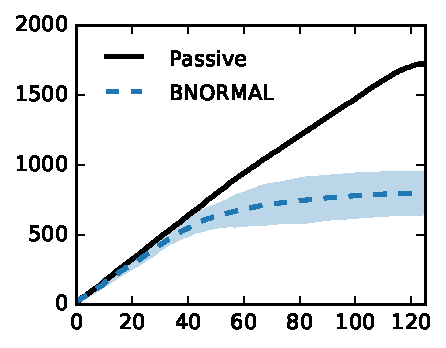
\includegraphics[width=0.42\linewidth]{images/toy_5_5_5.pdf}
	}
	\subfigure[E=10, K=10, D=5\label{fig:syn2}]{
	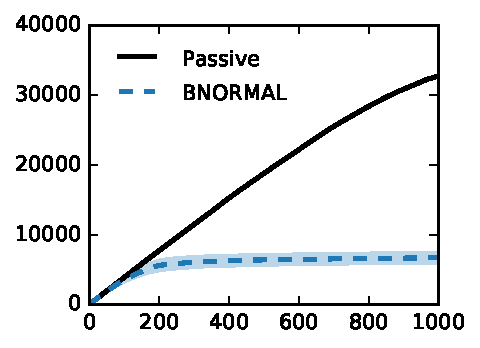
\includegraphics[width=0.45\linewidth]{images/toy_10_10_5.pdf}				
	}
%	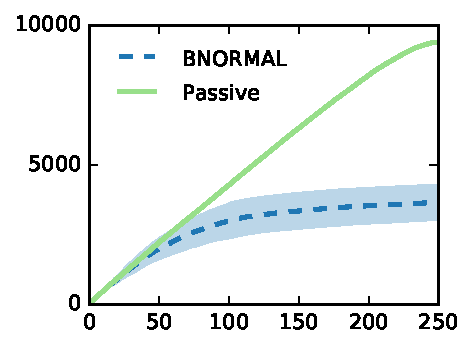
\includegraphics[width=0.32\linewidth]{images/toy_5_10_5.pdf}			
%	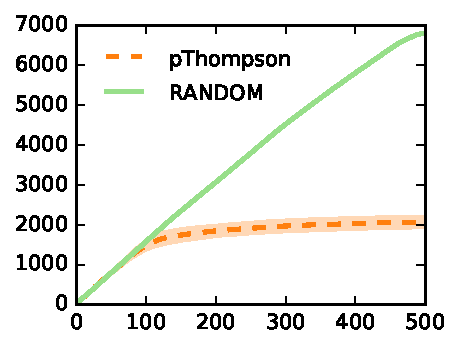
\includegraphics[width=0.32\linewidth]{images/toy_10_5_5.pdf}				
	\caption{\label{fig:synthetic} Cumulative regret of particle Thompson sampling on different sizes of the synthetic dataset. The synthetic dataset is generated by the model assumption (Eq. \ref{eqn:entity_gen} - \ref{eqn:triple_gen}). We compared the particle Thompson sampling with random sampling method. The averaged cumulative regrets are plotted with one standard error. As the model obtained more and more labeled samples from Thompson sampling, the cumulative regrets are converged. This result  indicates the particle sampling correctly inferred latent features of entities and relations on the synthetic datasets. // The results are averaged over 10 runs. $\sigma_e = 10$, $\sigma_r=10$, $\sigma_x=0.1$, $H=5$.}
\end{figure}


\subsection{particle Thompson sampling}
\begin{figure}[t]
	\centering
	
	\subfigure[KINSHIP]{
	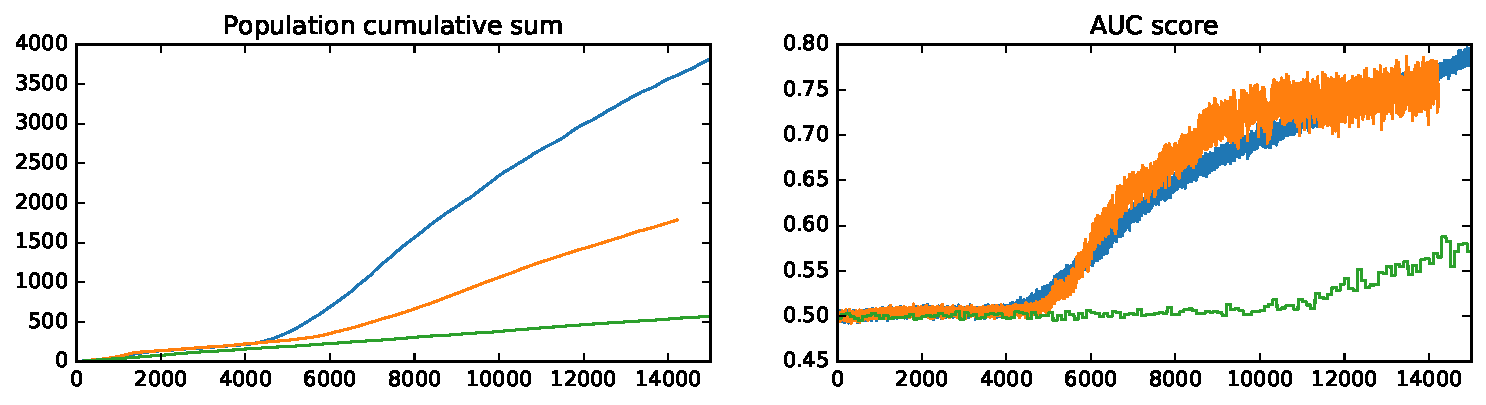
\includegraphics[width=\linewidth]{images/thompson_kinship.pdf}
	}
	\subfigure[UMLS]{
	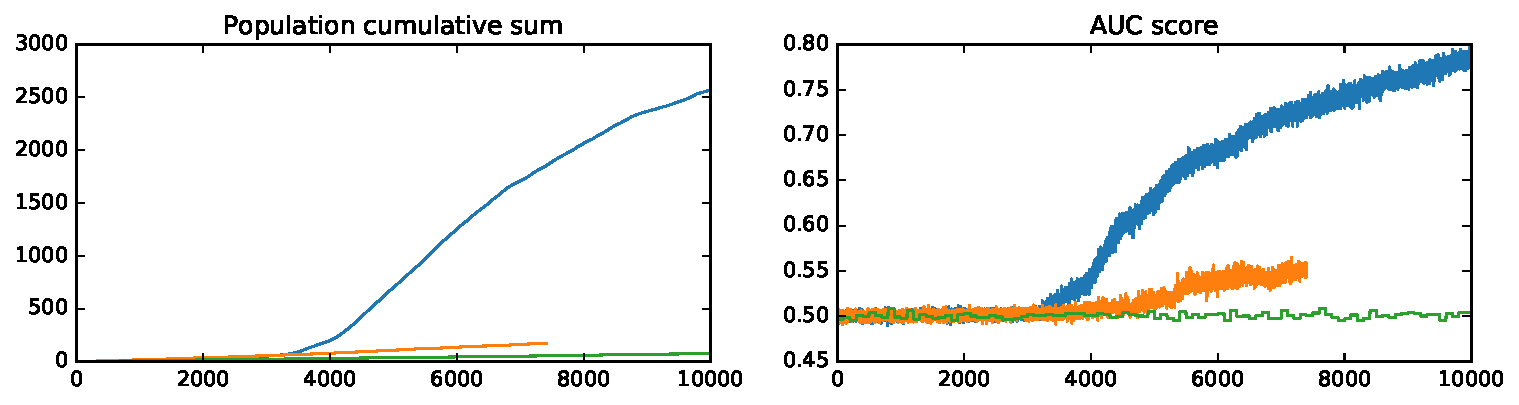
\includegraphics[width=\linewidth]{images/thompson_umls.pdf}				
	}
	\subfigure[NATION]{
	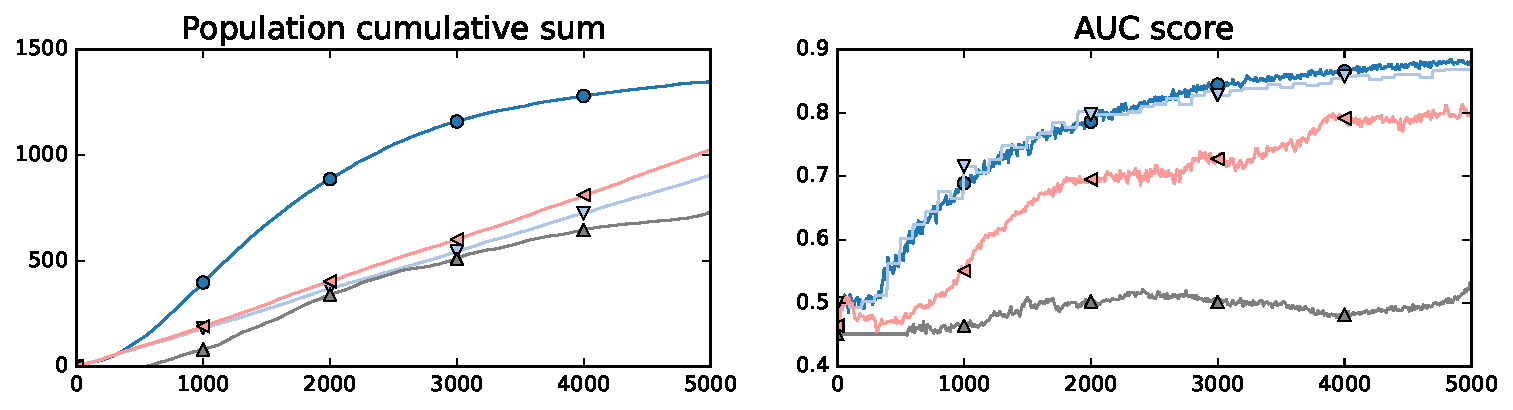
\includegraphics[width=\linewidth]{images/thompson_nation.pdf}				
	}	
	\caption{Placeholder for the future results. Will include the cumulative gain and ROC-AUC score of the developed models with the active and passive learning methods. We will see how the compositional model performs to compare with other models without any initial observation (May include the IBM model without any initial observation).}
\end{figure}

\subsection{Compositional ...}
\begin{figure}[t]
	\centering
	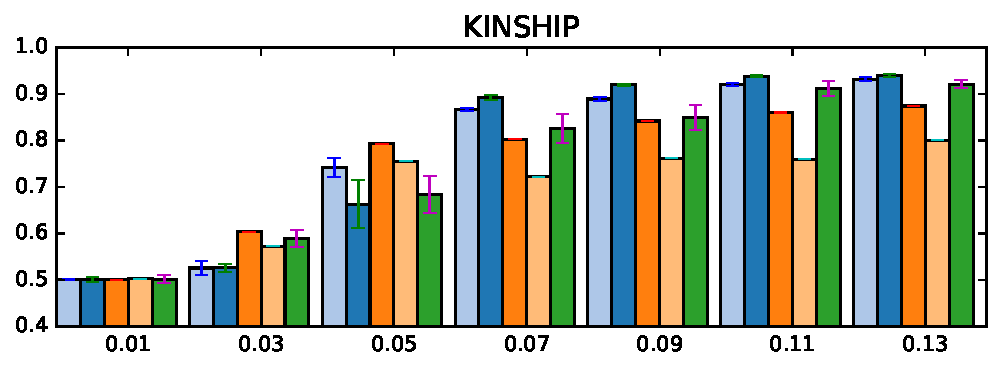
\includegraphics[width=\linewidth]{images/comp_training_error_kinship_small.pdf}
	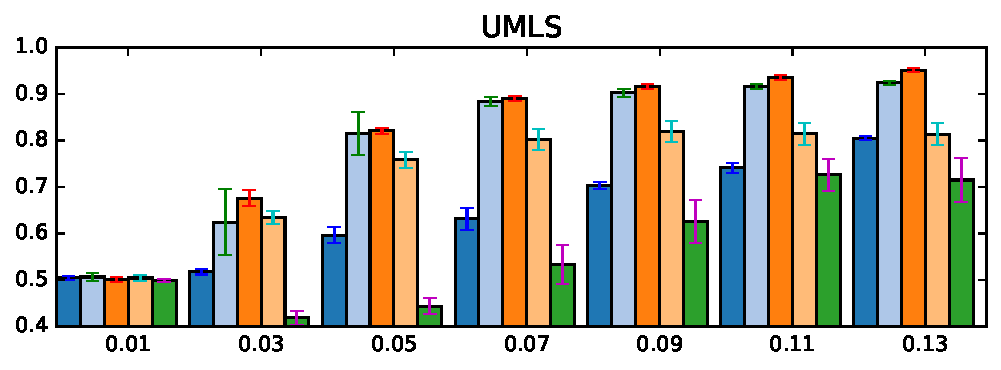
\includegraphics[width=\linewidth]{images/comp_training_error_umls_small.pdf}			
	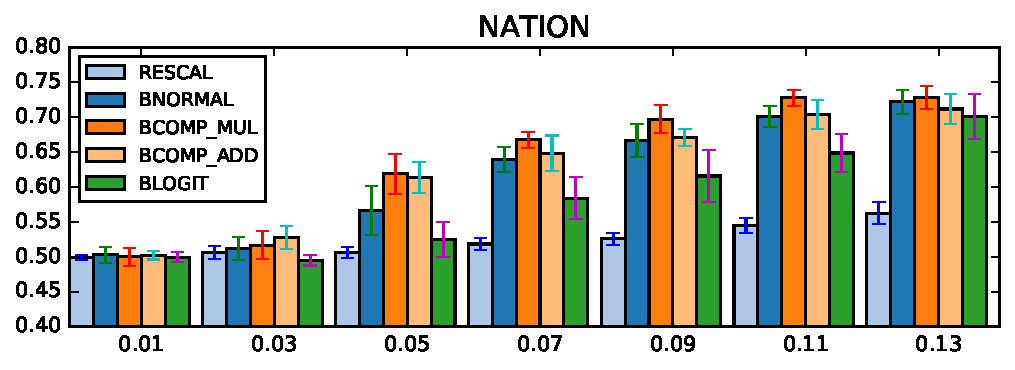
\includegraphics[width=\linewidth]{images/comp_training_error_nation_small.pdf}				
	\caption{\label{fig:r_vs_br} ROC-AUC scores of compositional models. The x-axis denotes the proportion of an observed triples including negative triples used for training models. We  use another 30\% of triples to evaluate the ROC-AUC score. In general, compositional models outperform BRESCAL and BLOGIT model when the size of training set is relatively small, whereas BRESCAL and BLOGIT perform slightly better than or comparable to the compositional models when the size of training set is relatively large. For UMLS dataset, the multiplicative compositional model consistently outperforms the other models across all training proportions.}
\end{figure} 

